% \VignetteDepends{MASS}
% \VignetteIndexEntry{NestedCohort Tutorial}
% \VignetteKeywords{Two-phase, Two-stage, Double Sampling, Case-Cohort, Nested Case-Control, Nested-Cohort}
% \VignettePackage{NestedCohort}

\documentclass[10pt]{article}
\usepackage{fullpage}
\usepackage{psfig}
\usepackage{S}
\usepackage{apalike}
\newcommand{\bex}{\begin{Example}}
  \newcommand{\eex}{\end{Example}}
                                % Use {Ex} for \large font S-PLUS code, {EXAMPLE} for \Huge
%%%
% Now on LaTeX 2e with documentclass and usepackage command!
%%%
% This is the old LaTeX 2.09 command.  If the above documentclass and
% usepackage commands don't work, comment them out and uncomment the
% documentstyle line and place at the top.
%\documentstyle[fullpage,psfig]{article}
%%%

\newenvironment{changemargin}[2]{\begin{list}{}{
         \setlength{\topsep}{0pt}\setlength{\leftmargin}{0pt}
         \setlength{\rightmargin}{0pt}
         \setlength{\listparindent}{\parindent}
         \setlength{\itemindent}{\parindent}
         \setlength{\parsep}{0pt plus 1pt}
         \addtolength{\leftmargin}{#1}\addtolength{\rightmargin}{#2}
         }\item }{\end{list}}
%    This environment takes two arguments, and will indent the left
%    and right margins by their values, respectively. Negative values
%    will cause the margins to be widened, so
%\begin{changemargin}{-1cm}{-1cm} widens the left and right margins
%    by 1cm.
%
%    However, this indents the first line of the region, I don't know why
%    hkatki 5/6/98

%\setlength{\textwidth}{7.5in}
%\setlength{\oddsidemargin}{-1.0in}
%\setlength{\evensidemargin}{-1.0in}
\usepackage{c:/R/R-2.5.1/share/texmf/Sweave}
\begin{document}           % End of preamble and beginning of text.


\title{Survival Analysis of Studies Nested within Cohorts using the NestedCohort Package}
\author{Hormuzd A. Katki and Steven D. Mark \\
Biostatistics Branch, Division of Cancer Epidemilogy and Genetics, NCI, NIH, DHHS \\
email: \texttt{katkih@mail.nih.gov}}
\date{\today}
\maketitle
\tableofcontents


\section{Overview}
\label{sec:overview}

The \texttt{NestedCohort} package provides functions that perform survival analysis (Cox
model and Kaplan-Meier) on studies nested within cohorts to estimate hazard ratios,
survival probabilities and attributable risks, all standardized for
confounders~\cite{Mark:Katki:06}.  

A study nested within a cohort is any cohort study on which a covariate is observed only
on a sample of all cohort members (call this covariate the exposure, to distinguish it
from covariates observed on the full cohort).  This is a special case of two-phase
studies: here the first phase is a cohort.  Typical examples are case-control studies
conducted within defined cohorts, nested case-control, or case-cohort studies.
NestedCohort is more general than these examples:
\begin{enumerate}
\item Allows cases to have missing exposures.  Standard nested case-control and
  case-cohort software can suffer from bias if cases are missing exposures.
\item Allows stratified sampling of subjects on whom the exposure is observed on.  Allows
  you to stratify on any variables available on all cohort members, thus allowing for
  frequency matching on confounders, or frequency counter-matching to improve efficiency.
  This non-representative sampling is properly accounted by specifying it as the sampling
  model.
\item Extracts efficiency out of auxiliary variables (available on all cohort members)
  that cannot be incorporated into the risk regression, like those on the causal pathway or
  any variable correlated with the missing exposures (e.g. ``surrogates'' for exposure).
\item The missing exposure need not be a single scalar exposure, but can be multiple
  exposures.  For hazard ratio estimation, covariates can be continuous or categorical.
\end{enumerate}
NestedCohort allows frequency matching on confounders and time, but does not currently
support fine matching on variables or time.

NestedCohort is most useful when you are interested in survival probabilities and
attributable risks.  But even if you are only interested in relative risks,
\texttt{NestedCohort} can more effciently estimate relative risks than standard
case-control analyses, because \texttt{NestedCohort} can use subjects with the missing
exposure (who provide information through the outcome and other covariates observed on
them), and can exploit auxiliary variables to increase efficiency.

In our example data~\cite{Abnet:05}, we observe the esophageal cancer outcome and survival
time on everyone, along with relevant confounders.  We are interested in the effect of
concentrations of various metals, especially zinc, on esophageal cancer.  But measuring
the metal concentrations requires precious esophageal biopsy tissue as well as a costly
measurement technique, so it is difficult and expensive to measure metal concentrations on
everyone.  Thus we measured concentrations of zinc (as well as iron, nickel, copper,
calcium, and sulphur) on a chosen sample of the cohort.  This sample oversampled the cases
and those with advanced baseline histologies (i.e. those most likely to become cases)
since these are the most informative subjects.  Due to cost and availability constraints,
less than 30\% of the cohort could be sampled, so it was impossible to sample even a
majority.  Although this study has no auxiliary variables, we show how to use them if they
were available.  For this example, \texttt{NestedCohort} will provide adjusted hazard
ratios, standardized survival probabilities and population attributable risks (PAR) for
the effect of zinc on esophageal cancer.


This document is a tutorial for using the \texttt{NestedCohort} package.  The package
consists of three functions:
\begin{enumerate}
\item \texttt{nested.km:} Estimates the Kaplan-Meier survival curve to the nested cohort
data.
\item \texttt{nested.coxph:} Fits the Cox model to the nested cohort study to estimate
hazard ratios.
\item \texttt{nested.stdsurv:} Fits Cox's Hazard Ratio model to the stratified nested
cohort study to estimate hazard ratios, standardized survival probabilities, and
Population Attributable Risk.
\end{enumerate}


\section{Case Study: Zinc and Esophageal Cancer dataset of~\cite{Abnet:05}}
\label{sec:case-study:-zinc}

We demonstrate the functionality of this package using the zinc and esophageal cancer
dataset~\cite{Abnet:05}.  The aim is to fit survival models to study the effect of zinc on
time until esophageal cancer.  To access the package and the data, type

\begin{Schunk}
\begin{Sinput}
> library(NestedCohort)
> data(zinc)
\end{Sinput}
\end{Schunk}

\texttt{NestedCohort} requires the \texttt{survival} package that comes with every R
system and also the \texttt{MASS} package that has to be downloaded from CRAN as part of
the \texttt{VR} bundle.  Install \texttt{VR} from the web from the Packages menu after
starting up R.

To get summary information on the variables available in the dataset, type:

\begin{Schunk}
\begin{Sinput}
> str(zinc)
\end{Sinput}
\begin{Soutput}
'data.frame':	431 obs. of  61 variables:
 $ id8        : int  10100012 10100123 10300066 10400038 10400106 10400245 10500252 10500267 10800011 10800049 ...
 $ sex        : Factor w/ 2 levels "Female","Male": 1 1 2 2 2 1 1 1 2 2 ...
 $ agepill    : int  53 54 54 44 44 43 49 48 41 61 ...
 $ agestr     : Factor w/ 3 levels "Age<=50","51<=Age<=60",..: 2 2 2 1 1 1 1 1 1 3 ...
 $ smoke      : Factor w/ 2 levels "Never","Ever": 1 1 1 1 1 1 1 1 1 2 ...
 $ drink      : Factor w/ 2 levels "Never","Ever": 1 1 2 2 1 1 1 1 2 2 ...
 $ anyhist    : Factor w/ 2 levels "No Family History",..: NA NA NA NA NA NA NA NA NA NA ...
 $ basehist   : Factor w/ 7 levels "Normal","Esophagitis",..: 1 1 1 1 3 2 1 1 1 1 ...
 $ dysp1      : int  1 1 1 1 3 2 1 1 1 1 ...
 $ dysp2      : int  0 0 0 0 1 0 0 0 0 0 ...
 $ mildysp    : Factor w/ 2 levels "Worst isn't mild",..: 1 1 1 1 2 1 1 1 1 1 ...
 $ moddysp    : Factor w/ 2 levels "Worst isn't moderate",..: 1 1 1 1 1 1 1 1 1 1 ...
 $ sevdysp    : Factor w/ 2 levels "Worst isn't severe",..: 1 1 1 1 1 1 1 1 1 1 ...
 $ ec01       : num  0 0 0 0 0 0 0 0 0 0 ...
 $ futime01   : int  5980 5980 5980 5980 5980 3404 5980 5980 5980 5980 ...
 $ zincset    : Factor w/ 2 levels "Unobserved Elements",..: 1 1 1 1 1 1 1 1 1 1 ...
 $ pcent      : num  NA NA NA NA NA NA NA NA NA NA ...
 $ scent      : num  NA NA NA NA NA NA NA NA NA NA ...
 $ cacent     : num  NA NA NA NA NA NA NA NA NA NA ...
 $ fecent     : num  NA NA NA NA NA NA NA NA NA NA ...
 $ nicent     : num  NA NA NA NA NA NA NA NA NA NA ...
 $ cucent     : num  NA NA NA NA NA NA NA NA NA NA ...
 $ zncent     : num  NA NA NA NA NA NA NA NA NA NA ...
 $ pqt        : int  NA NA NA NA NA NA NA NA NA NA ...
 $ sqt        : int  NA NA NA NA NA NA NA NA NA NA ...
 $ caqt       : int  NA NA NA NA NA NA NA NA NA NA ...
 $ feqt       : int  NA NA NA NA NA NA NA NA NA NA ...
 $ niqt       : int  NA NA NA NA NA NA NA NA NA NA ...
 $ cuqt       : int  NA NA NA NA NA NA NA NA NA NA ...
 $ znqt       : int  NA NA NA NA NA NA NA NA NA NA ...
 $ pq1        : int  NA NA NA NA NA NA NA NA NA NA ...
 $ pq2        : int  NA NA NA NA NA NA NA NA NA NA ...
 $ pq3        : int  NA NA NA NA NA NA NA NA NA NA ...
 $ pq4        : int  NA NA NA NA NA NA NA NA NA NA ...
 $ sq1        : int  NA NA NA NA NA NA NA NA NA NA ...
 $ sq2        : int  NA NA NA NA NA NA NA NA NA NA ...
 $ sq3        : int  NA NA NA NA NA NA NA NA NA NA ...
 $ sq4        : int  NA NA NA NA NA NA NA NA NA NA ...
 $ caq1       : int  NA NA NA NA NA NA NA NA NA NA ...
 $ caq2       : int  NA NA NA NA NA NA NA NA NA NA ...
 $ caq3       : int  NA NA NA NA NA NA NA NA NA NA ...
 $ caq4       : int  NA NA NA NA NA NA NA NA NA NA ...
 $ feq1       : int  NA NA NA NA NA NA NA NA NA NA ...
 $ feq2       : int  NA NA NA NA NA NA NA NA NA NA ...
 $ feq3       : int  NA NA NA NA NA NA NA NA NA NA ...
 $ feq4       : int  NA NA NA NA NA NA NA NA NA NA ...
 $ niq1       : int  NA NA NA NA NA NA NA NA NA NA ...
 $ niq2       : int  NA NA NA NA NA NA NA NA NA NA ...
 $ niq3       : int  NA NA NA NA NA NA NA NA NA NA ...
 $ niq4       : int  NA NA NA NA NA NA NA NA NA NA ...
 $ cuq1       : int  NA NA NA NA NA NA NA NA NA NA ...
 $ cuq2       : int  NA NA NA NA NA NA NA NA NA NA ...
 $ cuq3       : int  NA NA NA NA NA NA NA NA NA NA ...
 $ cuq4       : int  NA NA NA NA NA NA NA NA NA NA ...
 $ znq1       : int  NA NA NA NA NA NA NA NA NA NA ...
 $ znq2       : int  NA NA NA NA NA NA NA NA NA NA ...
 $ znq3       : int  NA NA NA NA NA NA NA NA NA NA ...
 $ znq4       : int  NA NA NA NA NA NA NA NA NA NA ...
 $ stdagepill : num  -0.182  0.000  0.000 -1.818 -1.818 ...
 $ znquartiles: Factor w/ 4 levels "Q1","Q2","Q3",..: NA NA NA NA NA NA NA NA NA NA ...
 $ observed   : num  0 0 0 0 0 0 0 0 0 0 ...
\end{Soutput}
\end{Schunk}

The survival time is \texttt{futime01} and the esophageal cancer outcome indicator is
\texttt{ec01}.  We want effect of zinc on time to esophageal cancer, and we will use the
variables \texttt{zncent} as the continuous zinc measure and \texttt{znquartiles} as a
factor variable of which quartile of the continuous zinc measure each subject falls into
(the quartile cutpoints are taken from the zinc levels in the controls).  The baseline
histology, which measures whether and how severe any precancerous lesions are, is the
variable \texttt{basehist}.


\section{Specifying the Sampling Model}
\label{sec:sampling-model}

\texttt{NestedCohort} requires you to specify the variables that determine the sampling
scheme for whom the missing exposure is observed on.  These variables account for the
sampling scheme by estimating the probability that each subject would would have their
exposure observed on them.  By default, this sampling probability is modeled with a
logistic regression of sampling status on the sampling variables.  The inverse of these
estimated sampling probabilities are used to weight each observation in the estimation of
the survival curves.  For details, see~\cite{Mark:Katki:06}.

To choose the sampling variables, note that any variable that has information about the
outcome or missing exposures is potentially worthwhile to sample on~\cite{Mark:Katki:06}.
Sampling on case/control status is almost always important: you should try to observe the
exposure on as many cases as possible.  For the zinc data, baseline esophageal histology
is a powerful potential confounder, as it is tightly linked to being a case, and if lack
of zinc causes esophageal cancer, then it may well cause precancerous lesions.  To control
for baseline histology, we chose to frequency match on it.  Here is our sampling scheme:

\begin{verbatim}
Baseline Histology   Case    Control   Total  
            Normal 14 / 22  17 / 221  31 / 243
       Esophagitis 19 / 26  22 /  82  41 / 108
    Mild Dysplasia 12 / 17  19 /  35  31 /  52
Moderate Dysplasia  3 /  7   4 /   6   7 /  13
  Severe Dysplasia  5 /  6   3 /   4   8 /  10
               CIS  2 /  2   0 /   0   2 /   2                               
               NOS  1 /  1   2 /   2   3 /   3                   
             Total 56 / 81  67 / 350 123 / 431
\end{verbatim}
Histology ranges from normal to ``CIS'' (carcinoma in-situ), with ``NOS'' meaning not
otherwise specified (histology undeterminable).  For each cell, the number to the right of
the slash is the total cohort members in that cell, the left is the number we sampled to
have zinc observed (i.e. in the top left cell, we measured zinc on 14 of the 22 members
who became cases and had normal histology at baseline).  Note that for each histology, we
sampled roughly 1:1 cases to controls (frequency matching), and we oversampled the more
severe histologies (who are more informative since they are more likely to become cases).
30\% of the cases could not be sampled.

This non-representative sampling will be accounted with inverse-probability weights by the
sampling model.  Since there are 7 baseline histologies, and case/control status, then the
sampling probability for each subject depends on which of 14 strata they belong to.  We
estimated the sampling fractions using a logistic model regressing having zinc
measurements on the 14 strata, allowing each stratum its own sampling fraction.  To do
this, each function will use the statement \texttt{samplingmod="ec01*basehist"}.

To be practical, the sampling design should not be so complex that it cannot be carried
out.  Also, the more sampling strata you choose, the more likely that an observation will
get a zero probability of having their exposure observed.  Every non-empty stratum must
have have someone sampled in it, or \texttt{NestedCohort} will not work.  To insure that
there is some sample in each stratum, you may have to collapse strata.  Also, if the
sampling is not under your direct control, then it is important that the sampling model
contain all covariates that could potentially affect whether the exposures are measured on
any subject.  For making valid estimates, \texttt{NestedCohort} depends on the sampling
model containing all variables used in the sampling scheme.  Finally,
\texttt{NestedCohort} does not support fine matching on variables or time.  However, you
can always include any frequency-matched variables (except for time) as covariates in the
analysis to further control for their effects.

Formally, missingness should not allowed for any variable in the sampling model.  However,
if there is missingness, for convenience, \texttt{NestedCohort} will remove from the
cohort any observations that have missingness in the sampling variables and will print a
warning to the user.  There should not be too many such observations.



\section{Kaplan-Meier Curves}
\label{sec:kaplan-meier-curves}

Let's first just look at the data by constructing non-parametric (Kaplan-Meier) survival
curves by quartile of zinc level using \texttt{nested.km}.  These Kaplan-Meier curves
have the usual interpretation: they do not standardize for other variables, and do not
account for competing risks.

To use this, you must provide a legal formula as per the \texttt{survfit} function and
also the sampling model to calculates stratum-specific sampling fractions.  To examine
survival from cancer within each quartile of zinc, and allowing different sampling
probabilities for each of the 14 strata above, use:

\begin{Schunk}
\begin{Sinput}
> mod <- nested.km(survfitformula = "Surv(futime01,ec01==1)~znquartiles", 
+     samplingmod = "ec01*basehist", exposureofinterest = "Q4", data = zinc)
\end{Sinput}
\begin{Soutput}
Risk Differences vs. znquartiles=Q4 by time 5980 
        Risk Difference  StdErr 95% CI Left 95% CI Right
Q4 - Q1         0.28175 0.10416     0.07760       0.4859
Q4 - Q2         0.05551 0.07566    -0.09278       0.2038
Q4 - Q3         0.10681 0.08074    -0.05143       0.2651
\end{Soutput}
\end{Schunk}

Note that the \texttt{survfitformula} and \texttt{samplingmod} require their arguments to
be inside double quotes.  The \texttt{data} argument is required, you must provide the
data frame within which all variables reside in.  This outputs the Kaplan-Meier curves
into a \texttt{survfit} object, so all the methods that are already there to manipulate
\texttt{survfit} objects can be used.

Running \texttt{nested.km} prints out a table of risk differences, the risk
differences will be towards the level named in \texttt{exposureofinterest}; in this case,
it's towards ``Q4'' which labels the 4th quartile of zinc concentration.  To look at the
estimated lifetables themselves to see the survival probabilities, use:
\begin{Schunk}
\begin{Sinput}
> summary(mod)
\end{Sinput}
\begin{Soutput}
Call: survfit(formula = as.formula(survfitformula), data = data, weights = 1/p.i.h.a.t., 
    na.action = na.omit, type = "fl")

308 observations deleted due to missingness 
                znquartiles=Q1 
 time n.risk n.event survival std.err lower 95% CI upper 95% CI
  163  125.5    1.37    0.989  0.0108        0.925        0.998
 1003  120.4    1.57    0.976  0.0169        0.906        0.994
 1036  118.8    1.00    0.968  0.0191        0.899        0.990
 1042  117.8    1.42    0.957  0.0227        0.881        0.985
 1056  116.4    1.37    0.945  0.0257        0.865        0.978
 1059  115.0    1.37    0.934  0.0284        0.849        0.972
 1064  113.7    1.37    0.923  0.0310        0.834        0.965
 1065  112.3    1.37    0.912  0.0333        0.818        0.958
 1067  110.9    1.42    0.900  0.0359        0.802        0.951
 1073  109.5    1.42    0.889  0.0382        0.786        0.944
 1075  108.1    1.57    0.876  0.0410        0.767        0.936
 1076  106.5    3.94    0.844  0.0468        0.725        0.915
 1181  102.6    1.42    0.832  0.0489        0.709        0.907
 1522  101.2    1.00    0.824  0.0503        0.698        0.901
 2247   96.4    1.37    0.813  0.0524        0.683        0.893
 2796   95.1    1.57    0.799  0.0550        0.664        0.885
 3059   91.6    1.42    0.787  0.0572        0.648        0.876
 3313   90.2    1.57    0.774  0.0597        0.629        0.867
 3433   88.7    1.57    0.760  0.0622        0.611        0.858
 4108   74.1    1.37    0.746  0.0646        0.593        0.849
 4154   72.7    1.57    0.730  0.0674        0.572        0.838
 4198   71.1    1.37    0.716  0.0699        0.553        0.828
 4370   69.8    1.20    0.704  0.0721        0.537        0.820
 4899   66.7    1.37    0.690  0.0748        0.518        0.811
 5674   63.5    1.37    0.675  0.0776        0.498        0.801
 5837   62.2    2.33    0.650  0.0830        0.463        0.786
 5893   59.8    1.57    0.633  0.0862        0.441        0.775

                znquartiles=Q2 
 time n.risk n.event survival std.err lower 95% CI upper 95% CI
 1038  116.9    1.57    0.987  0.0133        0.909        0.998
 1064  115.3    4.51    0.949  0.0260        0.864        0.981
 1070  110.8    2.33    0.929  0.0324        0.830        0.971
 1781   95.5    1.37    0.916  0.0358        0.811        0.964
 3144   68.1    1.42    0.897  0.0414        0.779        0.954
 3706   64.8    1.37    0.878  0.0468        0.748        0.944
 4139   63.5    1.37    0.859  0.0520        0.718        0.933

                znquartiles=Q3 
 time n.risk n.event survival std.err lower 95% CI upper 95% CI
  318  125.1    1.20    0.990 0.00948        0.934        0.999
  733  123.9    1.20    0.981 0.01340        0.926        0.995
 1001  122.7    1.37    0.970 0.01759        0.907        0.991
 1005  121.4    1.42    0.959 0.02130        0.888        0.985
 1046  120.0    2.62    0.938 0.02647        0.859        0.973
 1061  117.3    1.20    0.929 0.02841        0.847        0.968
 1919  114.8    1.42    0.917 0.03113        0.830        0.961
 2082  109.7    1.37    0.906 0.03390        0.812        0.954
 2247  108.3    2.33    0.886 0.03923        0.781        0.943
 2271  106.0    1.37    0.875 0.04164        0.765        0.936
 3144  102.7    1.57    0.862 0.04472        0.745        0.928
 3973   84.4    1.57    0.846 0.04853        0.721        0.918
 5294   66.2    1.57    0.826 0.05364        0.689        0.907
 5351   64.6    1.42    0.808 0.05800        0.662        0.896

                znquartiles=Q4 
 time n.risk n.event survival std.err lower 95% CI upper 95% CI
 1037   59.8    1.42    0.977  0.0235        0.840        0.997
 4143   44.4    1.42    0.946  0.0388        0.789        0.987
 5189   41.1    1.37    0.915  0.0514        0.736        0.975
\end{Soutput}
\end{Schunk}

The first line shows the actual \texttt{survfit} line that my program uses to create the
survival estimates, where NestedCohort computes the standard error estimates and plugs
them into the \texttt{survfit} object.  It then notes how many observations were
``deleted'' because of missing data -- this only includes those who have the covariates of
interest observed -- but the ''deleted'' observations still contribute to the final
estimates via estimation of the sampling probabilities.  Next is the lifetable for each
level of zinc, each line shows the time, the \underline{weighted} numbers of those at risk
and who had the developed cancer, the survival estmate at that time, its standard error,
and its confidence interval.  It's clear that those in the first vs. last quartile of zinc
have very different survival experiences.

The optional argument \texttt{outputsamplingmod} allows you to return the sampling model
that the sampling probabilities were calculated from.  It's important to examine this
model if you're warned that it didn't converge.  Note that if you included in the above
command, the option \texttt{outputsamplingmod=T}, then \texttt{nested.km} will output
into the object \texttt{mod} a list with 2 components, the \texttt{survmod} component
being the Kaplan-Meier \texttt{survfit} object, and the other \texttt{samplingmod}
component being the sampling model. To access a component, you have to use \$, so to
access the Kaplan-Meier curves, you would type \texttt{mod\$survmod}.  Similarly, the
optional argument \texttt{outputriskdiff} will keep the table of risk differences, which
can be accessed via \texttt{mod\$riskdiff}


\subsection{Plotting Kaplan-Meier Curves}
\label{sec:plott-kapl-meier}

To use the \texttt{plot} function for \texttt{survfit} objects, just use the commands as
shown in figure~\ref{fig:PlotKM}.

\begin{figure}
  \centering
\begin{Schunk}
\begin{Sinput}
> plot(mod, ymin = 0.6, xlab = "time", ylab = "survival", main = "Survival by Quartile of Zinc", 
+     legend.text = c("Q1", "Q2", "Q3", "Q4"), lty = 1:4, legend.pos = c(2000, 
+         0.7))
\end{Sinput}
\end{Schunk}
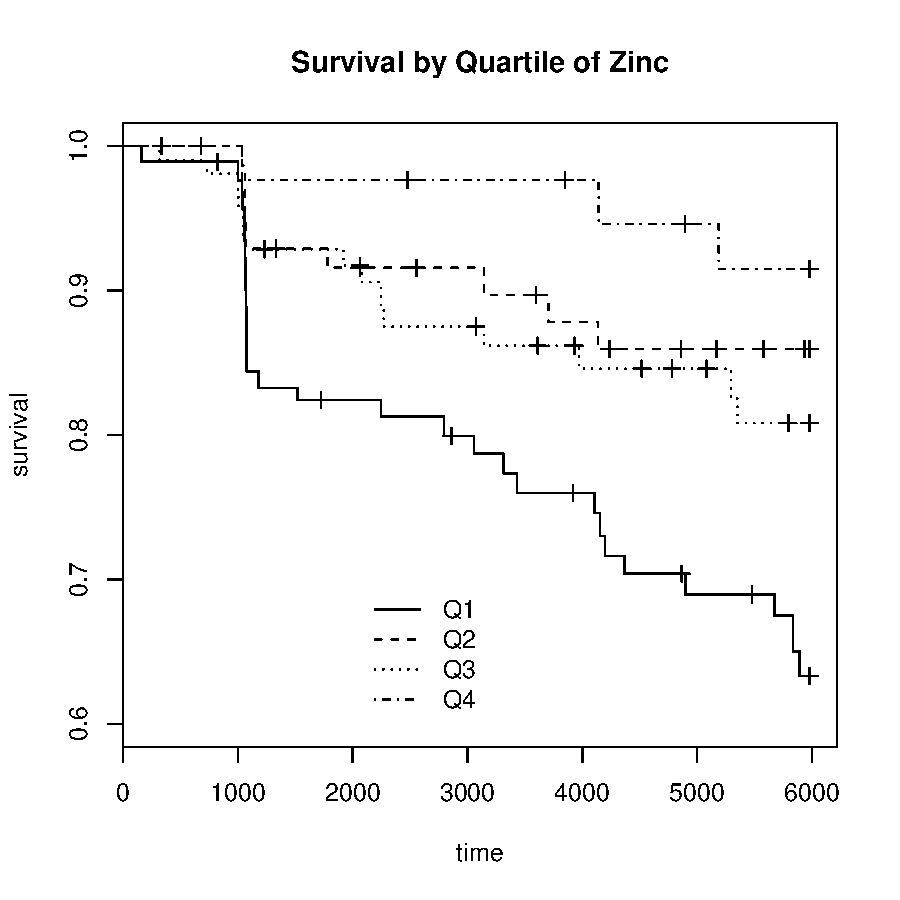
\includegraphics{NestedCohort-PlotKM}

\caption{Kaplan-Meier curves for cancer survival by each quantile of zinc}
\label{fig:PlotKM}
\end{figure}

You have a lot of control over the plot: use \texttt{ymin} to denote a reasonable smallest
survival value to get the best looking graph, then create the legend by telling what label
goes with each curve, giving the lines different types (\texttt{lty}) and the x-y
coordinates for positioning the the lower left corner of the legend.  Some other useful
options are \texttt{conf.int}, which if you set to \texttt{conf.int=T} will plot pointwise
confidence bands around each survival curve, and \texttt{mark.time}, which if you set to
\texttt{mark.time=T} will place a mark at each time where there are only censoring events
on each survival curve.

The \texttt{survfit} methods \texttt{plot,print,summary} all work with \texttt{nested.km}.
To all functions that work with \texttt{survfit} objects (but not necessarily with
\texttt{nested.km}) , type \texttt{help.start()} to open the HTML help, click search, and
type in \texttt{survfit} to bring up all the functions.

\texttt{nested.km} has some requirements:
\begin{enumerate}
\item It requires that all your variables be in a dataframe denoted by the \texttt{data}
  argument.
\item No variable in the dataframe can be named \texttt{o.b.s.e.r.v.e.d.} or
\texttt{p.i.h.a.t.}.
\item All variables in the \texttt{survfitformula} must be variables of type factor.
\item The \texttt{survfitformula} argument must be a valid formula for \texttt{survfit}
  objects -- so in particular note that terms with '+' in between them are automatically
  crossed to create strata (i.e. to plot the 4 survival curves by sex and smoking
  (ever/never) status, use \texttt{survfitformula=sex+smoke}), so that it is not necessary
  to use the '*' operator.
\item Currently does not allow staggered entry into the cohort.  The
  survival estimates will be correct, but their standard errors will be wrong.
\end{enumerate}


\subsection{Aside: Using \texttt{survfit} with weights}
\label{sec:texttts-with-weights}

The \texttt{survfit} function in the \texttt{survival} library uses weights, and in fact
\texttt{nested.km} uses \texttt{survfit} to estimate the survival curve.  However, the
standard errors reported by \texttt{survfit} are usually quite different from, and usually
much smaller than, the correct ones as reported by \texttt{nested.km}.



\section{Relative Risks (Hazard Ratios)}
\label{sec:relat-risks-hazard}

To estimate relative risks (i.e. hazard ratios) using the Cox model, use the function
\texttt{nested.coxph}.  \texttt{nested.coxph} relies on the function \texttt{coxph} that
is already in the \texttt{survival} package, and imitates its syntax as much as possible.

We are interested in estimating the effect of zinc (as \texttt{zncent}, a continuous
variable standardized to have nearly 0 median and where a 1 unit change is an increase of
1 quartile in zinc) on esophageal cancer, but controlling for sex, age (as
\texttt{agepill}, a continuous variable), smoking, drinking (both binary ever/never),
dysplasia grade (mild/moderate/severe), and family history (yes/no).  For the sampling
model, we use the same model of fitting a separate parameter to each of the
\texttt{ec01*basehist} sampling strata.  We do this with:

\begin{Schunk}
\begin{Sinput}
> coxmod <- nested.coxph(coxformula = "Surv(futime01,ec01==1)~sex+agepill+basehist+anyhist+zncent", 
+     samplingmod = "ec01*basehist", data = zinc)
> summary(coxmod)
\end{Sinput}
\begin{Soutput}
Call:
coxph(formula = as.formula(coxformula), data = data, weights = 1/p.i.h.a.t., 
    subset = TRUE, na.action = na.omit, control = coxphcontrol, 
    method = "breslow", robust = FALSE, x = TRUE)

  n=123 (308 observations deleted due to missingness)
                              coef exp(coef) se(coef)      z       p
sexMale                    -0.1854     0.831   0.3925 -0.472 6.4e-01
agepill                     0.0482     1.049   0.0266  1.809 7.1e-02
basehistEsophagitis         1.0909     2.977   0.3795  2.874 4.0e-03
basehistMild Dysplasia      1.5863     4.886   0.4086  3.882 1.0e-04
basehistModerate Dysplasia  1.9399     6.958   0.4958  3.913 9.1e-05
basehistSevere Dysplasia    2.4029    11.055   0.6052  3.970 7.2e-05
basehistNOS                 1.1097     3.033   1.1847  0.937 3.5e-01
basehistCIS                 3.5389    34.430   0.6140  5.764 8.2e-09
anyhistFamily History       0.2804     1.324   0.3876  0.723 4.7e-01
zncent                     -0.3134     0.731   0.1244 -2.519 1.2e-02

                           exp(coef) exp(-coef) lower .95 upper .95
sexMale                        0.831     1.2038     0.385     1.793
agepill                        1.049     0.9529     0.996     1.106
basehistEsophagitis            2.977     0.3359     1.415     6.263
basehistMild Dysplasia         4.886     0.2047     2.193    10.882
basehistModerate Dysplasia     6.958     0.1437     2.633    18.386
basehistSevere Dysplasia      11.055     0.0905     3.376    36.199
basehistNOS                    3.033     0.3297     0.298    30.930
basehistCIS                   34.430     0.0290    10.336   114.695
anyhistFamily History          1.324     0.7555     0.619     2.830
zncent                         0.731     1.3681     0.573     0.933

Rsquare= NA   (max possible= NA )
Likelihood ratio test= NA  on 10 df,   p=NA
Wald test            = 97.5  on 10 df,   p=2.22e-16
Score (logrank) test = NA  on 10 df,   p=NA
\end{Soutput}
\end{Schunk}

In this output, the first table shows log(hazard ratios) and inference, while the second
table shows the hazard ratio estimates themselves with their associated confidence
intervals.  For a quartile increase in zinc, there is about a 22.1\% decrease in the
hazard of esophageal cancer that has a p-value of 0.06.

The extra arguments \texttt{outputsamplingmod, glmlink, glmcontrol} work the same as for
\texttt{nested.km}.

\texttt{nested.coxph} has the following requirements:
\begin{enumerate}
\item It requires that all your variables be in a dataframe denoted by the \texttt{data}
argument.
\item No variable in the dataframe can be named \texttt{o.b.s.e.r.v.e.d.} or
\texttt{p.i.h.a.t.}.
\item Must use Breslow tie-breaking.
\item No \texttt{cluster} statements allowed.
\end{enumerate}

However, \texttt{nested.coxph} does allow staggered entry into the cohort, stratification
of the baselize hazard via \texttt{strata}, and use of \texttt{offset} arguments to
\texttt{coxph} (see help for \texttt{coxph} for more information).

If you have some sporadically missing values in other covariates not in the sampling
model, they will count as subjects with covariate vectors with some missingness.  The
sampling model has to account for missingness in those covariates also.  The sampling
model is really a model that regresses ``Any missing covariates in the covariate vector?''
on the sampling variables -- it's not particular to one covariate.  If this is just rare
nuisance missingness, you may want to remove these few subjects from the cohort.
\texttt{NestedCohort} does not warn you if you have sporadic missingness amongst Cox model
covariates.  However, the advantage of this is that you can fit multiple exposures with
missing values (see section~\ref{sec:how-fit-multiple}).



\section{Standardized Survival and Attributable Risks}
\label{sec:stand-surv-attr}

\texttt{nested.stdsurv} first estimates hazard ratios exactly like
\texttt{nested.coxph}, but then also estimates survival probabilities for each exposure
level as well as population attributable risks for a given exposure level, adjusting both
for confounders.  To do this, the usual right side of the formula for a Cox model must be
split in two pieces: the argument \texttt{exposures} denotes the part of the formula for
the exposures of interest, and this is joined with a '+' to \texttt{confounders} which
denotes the part of the formula for the confounders.  All variables in either part of the
formula must be categorical variables that inherit from class \texttt{factor}.  Note that
in either part, do not use '*' to mean interaction, use \texttt{interaction}.

In the zinc example, the exposures are \texttt{exposures="znquartiles"}, a factor variable
denoting which quartile of zinc each measurement is in.  This is only one variable, but
note that in general you can input a formula that includes all the exposures of interest.
The confounders are \texttt{confounders="sex+agestr+basehist+anyhist"}, these are the same
confounders in the hazard ratio example, except that we must categorize age as the factor
variable \texttt{agestr}.

In addition, the argument \texttt{timeofinterest} denotes the time at which survival
probabilities and attributable risks are to be calculated at, the default is at the last
event time.  The argument \texttt{exposureofinterest} is the name of the exposure level to
which the population is to be set at for computing the attributable risk; for zinc
\texttt{exposureofinterest="Q4"} denotes that we want an attributable risk estimate if we
could move the entire population's zinc levels into the fourth quartile of the current
zinc levels.  Finally, the argument \texttt{plot}, if set as \texttt{plot=T}, plots the
standardized survivals with 95\% confidence bounds at the time of interest and returns the
data used to make the plot.

Here is an example run, no plotting, with the zinc data:
\begin{Schunk}
\begin{Sinput}
> mod <- nested.stdsurv(outcome = "Surv(futime01,ec01==1)", exposures = "znquartiles", 
+     confounders = "sex+agestr+basehist+anyhist", samplingmod = "ec01*basehist", 
+     exposureofinterest = "Q4", data = zinc)
\end{Sinput}
\begin{Soutput}
Standardized Survival for znquartiles by time 5980 
      Survival  StdErr 95% CI Left 95% CI Right
Q1      0.5054 0.06936      0.3634       0.6312
Q2      0.7298 0.07768      0.5429       0.8501
Q3      0.6743 0.07402      0.5065       0.7959
Q4      0.9025 0.05262      0.7316       0.9669
Crude   0.7783 0.02283      0.7296       0.8194

Standardized Risk Differences vs. znquartiles = Q4 by time 5980 
           Risk Difference  StdErr 95% CI Left 95% CI Right
Q4 - Q1             0.3972 0.09008     0.22060       0.5737
Q4 - Q2             0.1727 0.09603    -0.01557       0.3609
Q4 - Q3             0.2282 0.08940     0.05294       0.4034
Q4 - Crude          0.1242 0.05405     0.01823       0.2301

PAR if everyone had znquartiles = Q4 
    Estimate StdErr 95% PAR CI Left 95% PAR CI Right
PAR   0.5602 0.2347         -0.2519           0.8455
\end{Soutput}
\end{Schunk}

The hazard ratio output is the same as for \texttt{nested.coxph}.  The next table shows
the survivals for each quartile of zinc that are standardized for all the confounders, as
well as the 'crude' survival, which is the observed survival in the population (so is not
standardized).  The next table shows the standardized survival differences vs. the
exposure of interest.  The last table shows the PAR, and the CI for PAR is based on the
log(1-PAR) transformation (this is often very different from, and superior to, the naive
CI without transformation).

The plot is in figure~\ref{fig:PlotStdSurv}.  This plots survival curves; to plot
cumulative incidence (1-survival), use \texttt{cuminc=T}.  The 95\% CI bars are plotted at
\texttt{timeofinterest}.  You can use any \texttt{plot} options in \texttt{plot}, in
particular, \texttt{main} to title the plot.
\begin{figure}
  \centering
\begin{Schunk}
\begin{Sinput}
> mod <- nested.stdsurv(outcome = "Surv(futime01,ec01==1)", exposures = "znquartiles", 
+     confounders = "sex+agestr+basehist+anyhist", samplingmod = "ec01*basehist", 
+     exposureofinterest = "Q4", plot = T, main = "Time to Esophageal Cancer by Quartiles of Zinc", 
+     data = zinc)
\end{Sinput}
\end{Schunk}
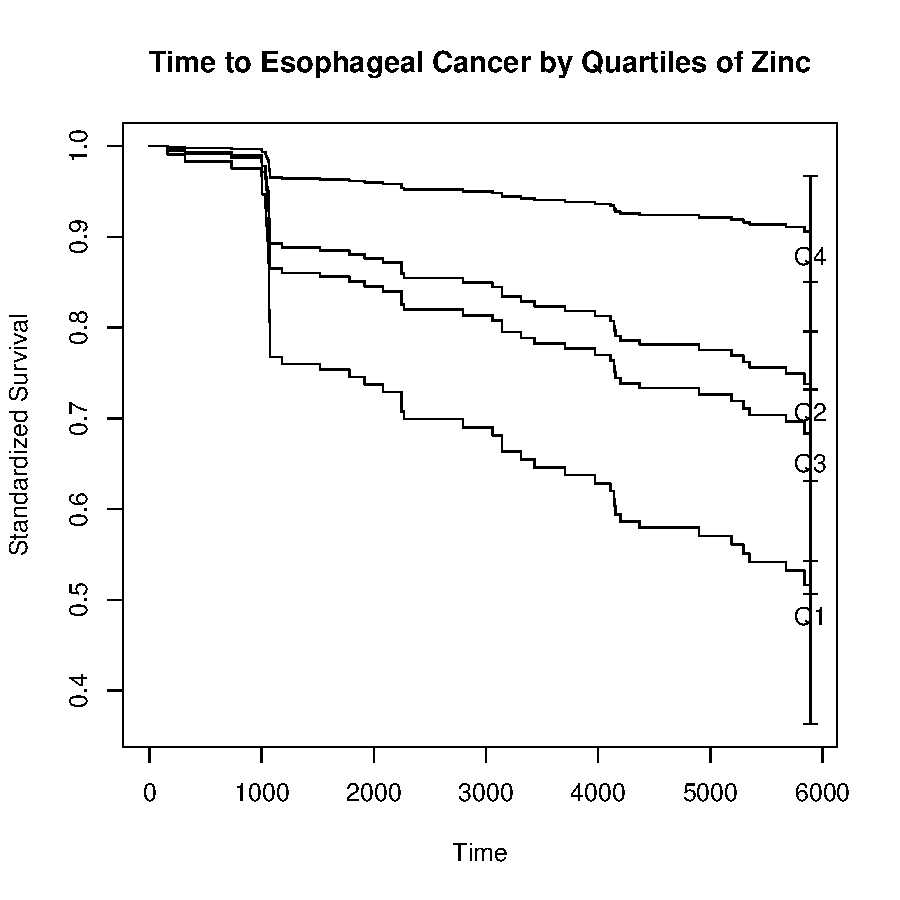
\includegraphics{NestedCohort-PlotStdSurv}
\caption{Survival curves for cancer survival by each quantile of zinc, standardized for confounders}
\label{fig:PlotStdSurv}
\end{figure}


\texttt{nested.stdsurv} has some requirements:
\begin{enumerate}
\item All your variables be in a dataframe denoted by the \texttt{data} argument.
\item No variable in the dataframe can be named \texttt{o.b.s.e.r.v.e.d.} or
\texttt{p.i.h.a.t.}.
\item The variables in the \texttt{exposures} and \texttt{confounders} must be variables
of type factor, even if they are binary.  In these formulas, never use '*' to mean
interaction, use \texttt{interaction}.
\item Currently does not allow staggered entry into the cohort.
\item Currently does not allow for the baseline hazard to be stratified via the
\texttt{strata} statement in a formula.  \texttt{cluser} and \texttt{offset} arguments are
not allowed either.
\item Only allows Breslow tie-breaking
\end{enumerate}




\section{Other topics}
\label{sec:other-topics}

\subsection{How to use auxiliary variables like surrogates or variables on the causal
  pathway}
\label{sec:how-use-auxiliary}

Auxiliary variables observed on the entire cohort cannot be used in the risk equation.
For example, auxiliaries might be surrogates for the exposure (for example, you may have a
cheap but rough measure of zinc available on everyone) or on the causal pathway between
exposure and outcome (for example, in studies of genetic polymorphisms and disease, family
history is a variable on a causal pathway from polymorphism to disease).  You cannot
include auxiliaries as covariates in the risk regression because they could distort the
association between exposure and disease, adjusted for confounders.  However, information
can be extracted out of auxiliaries by incorporating them in the sampling model.

Although the zinc dataset does not have any auxiliary variables, let's pretend we have a
categorical surrogate named znauxiliary observed on the full cohort.  You could sample
based on znauxiliary to get as wide a zinc distribution possible and thus improve
efficiency.  Clearly, you would then include znauxiliary as a sampling variable in the
sampling model:
\begin{verbatim}
samplingmod="ec01*basehist*znauxiliary"
\end{verbatim}

Even if you don't choose to sample based on znauxiliary, you can still include znauxiliary
in the sampling model as above.  This is because even though you don't explicitly sample
on it, if znauxiliary has something to do with zinc, and zinc has something to do with
either ec01 or basehist, you are implicitly sampling on znauxiliary.  The simulations
in~\cite{Mark:Katki:06} show the efficiency gain from including auxiliary variables in the
sampling model.  Including auxiliary variables will always reduce the standard errors of
the risk estimates.


\subsection{How to fit multiple exposures with missing values}
\label{sec:how-fit-multiple}

Multiple exposures (with missing values) are included in the risk regression just like any
other variable.  For example, if we want to estimate the esophageal cancer risk from zinc
and calcium jointly, the Cox model is:

\begin{Schunk}
\begin{Sinput}
> coxmod <- nested.coxph("Surv(futime01,ec01==1)~sex+agepill+basehist+anyhist+zncent+cacent", 
+     samplingmod = "ec01*basehist", data = zinc)
> summary(coxmod)
\end{Sinput}
\begin{Soutput}
Call:
coxph(formula = as.formula(coxformula), data = data, weights = 1/p.i.h.a.t., 
    subset = TRUE, na.action = na.omit, control = coxphcontrol, 
    method = "breslow", robust = FALSE, x = TRUE)

  n=123 (308 observations deleted due to missingness)
                              coef exp(coef) se(coef)      z       p
sexMale                    -0.1553     0.856   0.3974 -0.391 7.0e-01
agepill                     0.0438     1.045   0.0269  1.632 1.0e-01
basehistEsophagitis         1.0302     2.802   0.3962  2.600 9.3e-03
basehistMild Dysplasia      1.5692     4.803   0.4087  3.840 1.2e-04
basehistModerate Dysplasia  1.9079     6.739   0.5063  3.769 1.6e-04
basehistSevere Dysplasia    2.3442    10.425   0.6090  3.849 1.2e-04
basehistNOS                 1.1238     3.077   1.1658  0.964 3.4e-01
basehistCIS                 3.4673    32.050   0.6261  5.538 3.1e-08
anyhistFamily History       0.2775     1.320   0.3927  0.707 4.8e-01
zncent                     -0.3543     0.702   0.1306 -2.712 6.7e-03
cacent                      0.0918     1.096   0.1186  0.774 4.4e-01

                           exp(coef) exp(-coef) lower .95 upper .95
sexMale                        0.856     1.1680     0.393     1.866
agepill                        1.045     0.9571     0.991     1.101
basehistEsophagitis            2.802     0.3569     1.289     6.090
basehistMild Dysplasia         4.803     0.2082     2.156    10.699
basehistModerate Dysplasia     6.739     0.1484     2.498    18.176
basehistSevere Dysplasia      10.425     0.0959     3.160    34.394
basehistNOS                    3.077     0.3250     0.313    30.226
basehistCIS                   32.050     0.0312     9.396   109.325
anyhistFamily History          1.320     0.7576     0.611     2.850
zncent                         0.702     1.4252     0.543     0.906
cacent                         1.096     0.9123     0.869     1.383

Rsquare= NA   (max possible= NA )
Likelihood ratio test= NA  on 11 df,   p=NA
Wald test            = 102  on 11 df,   p=1.11e-16
Score (logrank) test = NA  on 11 df,   p=NA
\end{Soutput}
\end{Schunk}

If calcium were cut into quartiles into a variable named caquartiles, you can estimate the
standardized survival for all 16 combinations of znquartiles:

\begin{Schunk}
\begin{Sinput}
> zinc$caquartiles <- cut(zinc$cacent, breaks = quantile(zinc$cacent, 
+     seq(0, 1, 1/4), na.rm = T), include.lowest = T, labels = paste("Q", 
+     1:4, sep = ""))
> mod <- nested.stdsurv(outcome = "Surv(futime01,ec01==1)", exposures = "znquartiles+caquartiles", 
+     confounders = "sex+agestr+basehist+anyhist", samplingmod = "ec01*basehist", 
+     exposureofinterest = "Q4,Q4", data = zinc)
\end{Sinput}
\begin{Soutput}
Standardized Survival for znquartiles,caquartiles by time 5980 
      Survival  StdErr 95% CI Left 95% CI Right
Q1,Q1   0.5752 0.11064      0.3350       0.7560
Q1,Q2   0.4232 0.11319      0.2056       0.6267
Q1,Q3   0.5249 0.10823      0.2992       0.7087
Q1,Q4   0.4845 0.11811      0.2463       0.6874
Q2,Q1   0.7850 0.08645      0.5541       0.9055
Q2,Q2   0.6743 0.10748      0.4187       0.8367
Q2,Q3   0.7511 0.10194      0.4843       0.8931
Q2,Q4   0.7219 0.11873      0.4163       0.8859
Q3,Q1   0.7474 0.10953      0.4580       0.8971
Q3,Q2   0.6251 0.11247      0.3696       0.8011
Q3,Q3   0.7094 0.10872      0.4389       0.8666
Q3,Q4   0.6771 0.09071      0.4655       0.8197
Q4,Q1   0.9244 0.05029      0.7370       0.9800
Q4,Q2   0.8760 0.07789      0.6103       0.9651
Q4,Q3   0.9104 0.05240      0.7318       0.9722
Q4,Q4   0.8978 0.05977      0.6965       0.9684
Crude   0.7811 0.02265      0.7328       0.8218

Standardized Risk Differences vs. znquartiles,caquartiles = Q4,Q4 by time 5980 
              Risk Difference  StdErr 95% CI Left 95% CI Right
Q4,Q4 - Q1,Q1         0.32256 0.13258    0.062698      0.58243
Q4,Q4 - Q1,Q2         0.47454 0.13160    0.216613      0.73247
Q4,Q4 - Q1,Q3         0.37283 0.13511    0.108011      0.63765
Q4,Q4 - Q1,Q4         0.41329 0.11706    0.183852      0.64273
Q4,Q4 - Q2,Q1         0.11278 0.10894   -0.100739      0.32629
Q4,Q4 - Q2,Q2         0.22344 0.12466   -0.020902      0.46778
Q4,Q4 - Q2,Q3         0.14670 0.12528   -0.098855      0.39226
Q4,Q4 - Q2,Q4         0.17582 0.12037   -0.060094      0.41174
Q4,Q4 - Q3,Q1         0.15038 0.13155   -0.107450      0.40822
Q4,Q4 - Q3,Q2         0.27267 0.13303    0.011943      0.53340
Q4,Q4 - Q3,Q3         0.18840 0.13494   -0.076081      0.45288
Q4,Q4 - Q3,Q4         0.22066 0.09615    0.032215      0.40911
Q4,Q4 - Q4,Q1        -0.02667 0.04559   -0.116022      0.06269
Q4,Q4 - Q4,Q2         0.02180 0.05503   -0.086050      0.12965
Q4,Q4 - Q4,Q3        -0.01261 0.04426   -0.099359      0.07413
Q4,Q4 - Crude         0.11664 0.06146   -0.003824      0.23710

PAR if everyone had znquartiles,caquartiles = Q4,Q4 
    Estimate StdErr 95% PAR CI Left 95% PAR CI Right
PAR   0.5329 0.2719         -0.4616           0.8507
\end{Soutput}
\end{Schunk}

If however, there is an interaction between zinc and calcium, you will need to define the
exposure as:
\begin{verbatim}
exposures="interaction(znquartiles,caquartiles)"
\end{verbatim}


With multiple exposures, the key is to make sure that the missingness pattern is monotone.
In a monotone pattern, the exposures with missing values are entirely observed for some
people, and on others are entirely unobserved.  This is the case in this study, as the
zinc, iron, nickel, copper, calcium, and sulphur were all measured simultaneously on the
same subjects and none were measured on the others.  NestedCohort is designed to work for
monotone missingness.

In a non-monotone pattern, some subjects would have zinc observed but not calcium, and
vice versa, with few having both observed.  NestedCohort would treat the subjects who have
both measurements as the complete data, and all the others as missing data.  If the
non-monotonicity is small so that there are many cohort members with all measurements,
NestedCohort will still provide valid estimates and inference.  But if there is serious
non-monotonicity so that few cohort members have all the exposures observed on them, a
different technique, such as multiple imputation, may be better to use.


\subsection{Full cohort analysis}
\label{sec:full-cohort-analysis}

If all covariates are observed on the full cohort, you can still use NestedCohort to
estimate the survival and attributable risks.  In this case, set
\verb+samplingModel=''1''+, this will force equal weights for all cohort members, and
thus the weights don't come into play.  \texttt{nested.km} will work exactly as
\texttt{survfit} does. 

The Cox model standard errors provided by NestedCohort will not be the usual estimates
that you get out of \texttt{coxph} that depend on the model being properly specified.
Instead, NestedCohort will provide standard errors that are robust to model
misspecification.  These standard errors may be larger than the usual estimates.  These
robust standard errors will be used by \texttt{nested.stdsurv} to compute the CI for
standardized absolute and attributable risks.


\subsection{Importing data into R from plain text, SAS, Stata, or Excel}
\label{sec:importing-data-into}

For plain text, use the function \texttt{read.table}.  The \texttt{header=T} option takes
column names and makes them the column names in your data frame.

For SAS or Stata, you need install the foreign package from CRAN (in the same way you
installed the VR bundle).  To import Stata binary files, use \texttt{read.dta}.

For a SAS dataset (extension *.ssd0x or *.sas7bdat), use the function \texttt{read.ssd};
note that this function will actually run SAS on your computer to do its job.  However,
I've had trouble with this function.  Instead, I convert the SAS dataset into xport format
and then import the xport file.  For example, to convert hormuzd.sas7bdat into
htlv.xpt, I run the following SAS code:
\begin{verbatim}
libname src2rd V8 'E:\hkatki';
libname rd xport 'E:\hkatki\htlv.xpt' ;
options VALIDVARNAME=V6; * Need to truncate variable names, so variable names do change;
proc copy in=src2rd out=rd;
select hormuzd; * This is the name of the dataset;
run;
\end{verbatim}
To bring the xport file to R I use
\begin{verbatim}
htlv <- read.xport("htlv.xpt")
\end{verbatim}
\texttt{read.xport} does not need to run SAS.

To read from Excel, you need to install the gdata package and use \texttt{read.xls}.  This
function requires perl to be installed on your computer.


\begin{thebibliography}{}

\bibitem[Abnet et~al., 2005]{Abnet:05}
Abnet, C.~C., Lai, B., Qiao, Y.-L., Vogt, S., Luo, X.-M., Taylor, P.~R., Dong,
  Z.-W., Mark, S.~D., and Dawsey, S.~M. (2005).
\newblock Zinc concentration in esophageal biopsies measured by x-ray
  fluorescence and cancer risk.
\newblock {\em Journal of the National Cancer Institute}, 97(4):301--306.

\bibitem[Mark and Katki, 2006]{Mark:Katki:06}
Mark, S.~D. and Katki, H.~A. (2006).
\newblock Specifying and implementing nonparametric and semiparametric survival
  estimators in two-stage (sampled) cohort studies with missing case data.
\newblock {\em Journal of the American Statistical Association},
  101(474):460--471.

\end{thebibliography}


\end{document}

% This is the first package we are aware of that allows easy estimation of standardized
% absolute and attributable risks for nested cohort studies, and also the the first package
% that properly allows for stratified sampling of members into the
% subcohort.\footnote{Although~\cite{Bar94} and~\cite{Bar99} discuss stratified sampling,
% their sample SAS code \texttt{robphreg} does not allow for it.}


% In the simple case-cohort design, the survival outcomes of interest along with some
% covariates are measured on all cohort members, and the covariate of interest is measured
% on all cases and a simple random subsample of the cohort members.  The stratified
% case-cohort study generalizes the simple case-cohort design so that the subsampling scheme
% can be stratified on any information available on all cohort members: this includes any
% covariate, any surrogate variable for exposure, and case/control status (but excludes the
% outcome event time).  We also allow the covariate of interest to be multiple covariates,
% so you can examine multiple exposures simulataneously.  \texttt{NestedCohort} is based on
% the work of~\cite{Mark03} that is valid in much more general situations.


% Note that the stratified nested cohort design allows for subsampling the cases (i.e. it
% does not require that all cases have the covariate of interest measured on them), and
% allows for different sampling fractions between the strata.  The stratification allows you
% to oversample the most informative study subjects, thus increasing efficiency over the
% simple nested cohort design.  It is important to note that standard nested cohort analysis
% software will not provide correct estimates because they cannot handle stratified sampling
% nor subsampling of cases.


% Finally, our stratified nested cohort design encompasses not only the usual problem where
% confounders are observed on all subjects and the exposure observed on only the subsample,
% but also when a cheap surrogate for the exposure of interest is observed on all subjects,
% but the gold standard exposure assessment is available on only the subsample.  For
% example, let's say if we could estimate zinc concentration by estimating zinc intake from
% food frequency questionnaires, and this inexpensive measurement were available on all
% cohort members.  The gold-standard zinc measurement is observed on only a subsample.
% \texttt{NestedCohort} can estimate the risks associated with the gold-standard zinc.
% (I'D LIKE TO MAKE UP SOME FICTITIOUS MEASURE OF ZINC OBSERVED ON EVERYONE, THEN FIT THIS
% MODEL)

% Another important point is that no subject is allowed to have zero sampling probability --
% all subjects must have some chance of having their covariates of interest observed.  In
% particular, there cannot be any sampling strata where nobody has their covariates of
% interest observed.  When designing the study, you must insure that this does not happen.
% Note that if in some stratum only a tiny fraction are sampled, then although the risk
% estimates remain asymptotically valid, the risk estimates may be unstable in your finite
% sample and the asymptotic p-values and confidence intervals could be misleading.

